\documentclass[aspectratio=1610,onlymath]{beamer}
% \documentclass[aspectratio=1610,onlymath,handout]{beamer}

% Macros used by all lectures, but not necessarily by excercises

%%% General setup and dependencies:

% \usetheme[ddcfooter,nosectionnum]{tud}
\usetheme[nosectionnum,pagenum,noheader]{tud}
% \usetheme[nosectionnum,pagenum]{tud}

% Increase body font size to a sane level:
\let\origframetitle\frametitle
% \renewcommand{\frametitle}[1]{\origframetitle{#1}\normalsize}
\renewcommand{\frametitle}[1]{\origframetitle{#1}\fontsize{10pt}{13.2}\selectfont}
\setbeamerfont{itemize/enumerate subbody}{size=\small} % tud defaults to scriptsize!
\setbeamerfont{itemize/enumerate subsubbody}{size=\small}
% \setbeamerfont{normal text}{size=\small}
% \setbeamerfont{itemize body}{size=\small}

\renewcommand{\emph}[1]{\textbf{#1}}

\def\arraystretch{1.3}% Make tables even less cramped vertically

\usepackage[ngerman]{babel}
\usepackage[utf8]{inputenc}
\usepackage[T1]{fontenc}

%\usepackage{graphicx}
\usepackage[export]{adjustbox} % loads graphicx
\usepackage{import}
\usepackage{stmaryrd}
\usepackage[normalem]{ulem} % sout command
% \usepackage{times}
\usepackage{txfonts}

% \usepackage[perpage]{footmisc} % reset footnote counter on each page -- fails with beamer (footnotes gone)
\usepackage{perpage}  % reset footnote counter on each page
\MakePerPage{footnote}

\usepackage{tikz}
\usetikzlibrary{arrows,positioning}
% Inspired by http://www.texample.net/tikz/examples/hand-drawn-lines/
\usetikzlibrary{decorations.pathmorphing}
\pgfdeclaredecoration{penciline}{initial}{
    \state{initial}[width=+\pgfdecoratedinputsegmentremainingdistance,
    auto corner on length=1mm,]{
        \pgfpathcurveto%
        {% From
            \pgfqpoint{\pgfdecoratedinputsegmentremainingdistance}
                      {\pgfdecorationsegmentamplitude}
        }
        {%  Control 1
        \pgfmathrand
        \pgfpointadd{\pgfqpoint{\pgfdecoratedinputsegmentremainingdistance}{0pt}}
                    {\pgfqpoint{-\pgfdecorationsegmentaspect
                     \pgfdecoratedinputsegmentremainingdistance}%
                               {\pgfmathresult\pgfdecorationsegmentamplitude}
                    }
        }
        {%TO 
        \pgfpointadd{\pgfpointdecoratedinputsegmentlast}{\pgfpoint{1pt}{1pt}}
        }
    }
    \state{final}{}
}
\tikzset{handdrawn/.style={decorate,decoration=penciline}}
\tikzset{every shadow/.style={fill=none,shadow xshift=0pt,shadow yshift=0pt}}
% \tikzset{module/.append style={top color=\col,bottom color=\col}}

% Use to make Tikz attributes with Beamer overlays
% http://tex.stackexchange.com/a/6155
\tikzset{onslide/.code args={<#1>#2}{%
  \only<#1| handout:0>{\pgfkeysalso{#2}} 
}}
\tikzset{onslideprint/.code args={<#1>#2}{%
  \only<#1>{\pgfkeysalso{#2}} 
}}

%%% Title -- always set this first

\newcommand{\defineTitle}[3]{
	\newcommand{\lectureindex}{#1}
	\title{Formale Systeme}
	\subtitle{\href{\lectureurl}{#1. Vorlesung: #2}}
	\author{\href{http://korrekt.org/}{Markus Kr\"{o}tzsch}}
%	\author{\href{http://www.sebastian-rudolph.de}{Sebastian Rudolph} in Vertretung von \href{http://korrekt.org/}{Markus Kr\"{o}tzsch}}
	\date{#3}
	\datecity{TU Dresden}
% 	\institute{Computational Logic}
}

%%% Table of contents:

\RequirePackage{ifthen}

\newcommand{\highlight}[2]{%
	\ifthenelse{\equal{#1}{\lectureindex}}{\alert{#2}}{#2}%
}

\def\myspace{-0.7ex}
\newcommand{\printtoc}{
\begin{tabular}{r@{$\quad$}l}
\highlight{1}{1.} & \highlight{1}{Willkommen/Einleitung formale Sprachen}\\[\myspace]
\highlight{2}{2.} & \highlight{2}{Grammatiken und die Chomsky-Hierarchie}\\[\myspace]
\highlight{3}{3.} & \highlight{3}{Endliche Automaten}\\[\myspace]
\highlight{4}{4.} & \highlight{4}{Complexity of FO query answering}\\[\myspace]
\highlight{5}{5.} & \highlight{5}{Conjunctive queries}\\[\myspace]
\highlight{6}{6.} & \highlight{6}{Tree-like conjunctive queries}\\[\myspace]
\highlight{7}{7.} & \highlight{7}{Query optimisation}\\[\myspace]
\highlight{8}{8.} & \highlight{8}{Conjunctive Query Optimisation / First-Order~Expressiveness}\\[\myspace]
\highlight{9}{9.} & \highlight{9}{First-Order~Expressiveness / Introduction to Datalog}\\[\myspace]
\highlight{10}{10.} & \highlight{10}{Expressive Power and Complexity of Datalog}\\[\myspace]
\highlight{11}{11.} & \highlight{11}{Optimisation and Evaluation of Datalog}\\[\myspace]
\highlight{12}{12.} & \highlight{12}{Evaluation of Datalog (2)}\\[\myspace]
\highlight{13}{13.} & \highlight{13}{Graph Databases and Path Queries}\\[\myspace]
\highlight{14}{14.} & \highlight{14}{Outlook: database theory in practice}
\end{tabular}
}

\newcommand{\overviewslide}{%
\begin{frame}\frametitle{Overview}
\printtoc
\medskip

Siehe \href{\lectureurl}{course homepage [$\Rightarrow$ link]} for more information and materials
\end{frame}
}

%%% Colours:

\usepackage{xcolor,colortbl}
\definecolor{redhighlights}{HTML}{FFAA66}
\definecolor{lightblue}{HTML}{55AAFF}
\definecolor{lightred}{HTML}{FF5522}
\definecolor{lightpurple}{HTML}{DD77BB}
\definecolor{lightgreen}{HTML}{55FF55}
\definecolor{darkred}{HTML}{CC4411}
\definecolor{darkblue}{HTML}{176FC0}%{1133AA}
\definecolor{nightblue}{HTML}{2010A0}%{1133AA}
\definecolor{alert}{HTML}{176FC0}
\definecolor{darkgreen}{HTML}{36AB14}
\definecolor{strongyellow}{HTML}{FFE219}
\definecolor{devilscss}{HTML}{666666}

\newcommand{\redalert}[1]{\textcolor{darkred}{#1}}

%%% Style commands

\newcommand{\quoted}[1]{\texttt{"}{#1}\texttt{"}}
\newcommand{\squote}{\texttt{"}} % straight quote
\newcommand{\Sterm}[1]{\ensuremath{\mathtt{\textcolor{purple}{#1}}}}    % letters in alphabets
\newcommand{\Snterm}[1]{\textsf{\textcolor{darkblue}{#1}}} % nonterminal symbols
\newcommand{\Sntermsub}[2]{\Snterm{#1}_{\Snterm{#2}}} % nonterminal symbols
\newcommand{\Slang}[1]{\textbf{\textcolor{black}{#1}}}    % languages
\newcommand{\Slangsub}[2]{\Slang{#1}_{\Slang{#2}}}    % languages
% Code
\newcommand{\Scode}[1]{\textbf{#1}}    % reserved words in program listings, e.g., "if"
\newcommand{\Scodelit}[1]{\textcolor{purple}{#1}}    % literals in program listings, e.g., strings
\newcommand{\Scomment}[1]{\textcolor{gray}{#1}}    % comment in program listings

\newcommand{\epstrastar}{\mathrel{\mathord{\stackrel{\epsilon}{\to}}{}^*}} % transitive reflexive closure of epsilon transitions in an epslion-NFA

\newcommand{\narrowcentering}[1]{\mbox{}\hfill#1\hfill\mbox{}}

\newcommand{\defeq}{\mathrel{:=}}

\newcommand{\Smach}[1]{\ensuremath{\mathcal{#1}}}    % machines

%%% Slide layout commands:

\newcommand{\sectionSlide}[1]{
\frame{\begin{center}
\LARGE
#1
\end{center}}
}
\newcommand{\sectionSlideNoHandout}[1]{
\frame<handout:0>{\begin{center}
\LARGE
#1
\end{center}}
}

\newcommand{\mydualbox}[3]{%
 \begin{minipage}[t]{#1}
 \begin{beamerboxesrounded}[upper=block title,lower=block body,shadow=true]%
    {\centering\usebeamerfont*{block title}#2}%
    \raggedright%
    \usebeamerfont{block body}
%     \small
    #3%
  \end{beamerboxesrounded}
  \end{minipage}
}
% 
\newcommand{\myheaderbox}[2]{%
 \begin{minipage}[t]{#1}
 \begin{beamerboxesrounded}[upper=block title,lower=block title,shadow=true]%
    {\centering\usebeamerfont*{block title}\rule{0pt}{2.6ex} #2}%
  \end{beamerboxesrounded}
  \end{minipage}
}

\newcommand{\mycontentbox}[2]{%
 \begin{minipage}[t]{#1}%
 \begin{beamerboxesrounded}[upper=block body,lower=block body,shadow=true]%
    {\centering\usebeamerfont*{block body}\rule{0pt}{2.6ex}#2}%
  \end{beamerboxesrounded}
  \end{minipage}
}

\newcommand{\mylcontentbox}[2]{%
 \begin{minipage}[t]{#1}%
 \begin{beamerboxesrounded}[upper=block body,lower=block body,shadow=true]%
    {\flushleft\usebeamerfont*{block body}\rule{0pt}{2.6ex}#2}%
  \end{beamerboxesrounded}
  \end{minipage}
}

% label=180:{\rotatebox{90}{{\footnotesize\textcolor{darkgreen}{Beispiel}}}}
% \hspace{-8mm}\ghost{\raisebox{-7mm}{\rotatebox{90}{{\footnotesize\textcolor{darkgreen}{Beispiel}}}}}\hspace{8mm}
\newcommand{\examplebox}[1]{%
	\begin{tikzpicture}[decoration=penciline, decorate]
		\pgfmathsetseed{1235}
		\node (n1) [decorate,draw=darkgreen, fill=darkgreen!10,thick,align=left,text width=\linewidth, inner ysep=2mm, inner xsep=2mm] at (0,0) {#1};
% 		\node (n2) [align=left,text width=\linewidth,inner sep=0mm] at (n1.92) {{\footnotesize\raisebox{3mm}{\textcolor{darkgreen}{Beispiel}}}};
% 		\node (n2) [decorate,draw=darkgreen, fill=darkgreen!10,thick, align=left,text width=\linewidth,inner sep=2mm] at (n1.90) {{\footnotesize\raisebox{0mm}{\textcolor{darkgreen}{Beispiel}}}};
	\end{tikzpicture}%
}%

\newcommand{\codebox}[1]{%
	\begin{tikzpicture}[decoration=penciline, decorate]
		\pgfmathsetseed{1236}
		\node (n1) [decorate,draw=strongyellow, fill=strongyellow!10,thick,align=left,text width=\linewidth, inner ysep=2mm, inner xsep=2mm] at (0,0) {#1};
	\end{tikzpicture}%
}%

\newcommand{\defbox}[1]{%
	\begin{tikzpicture}[decoration=penciline, decorate]
		\pgfmathsetseed{1237}
		\node (n1) [decorate,draw=darkred, fill=darkred!10,thick,align=left,text width=\linewidth, inner ysep=2mm, inner xsep=2mm] at (0,0) {#1};
	\end{tikzpicture}%
}%

\newcommand{\theobox}[1]{%
	\begin{tikzpicture}[decoration=penciline, decorate]
		\pgfmathsetseed{1240}
		\node (n1) [decorate,draw=darkblue, fill=darkblue!10,thick,align=left,text width=\linewidth, inner ysep=2mm, inner xsep=2mm] at (0,0) {#1};
	\end{tikzpicture}%
}%

\newcommand{\anybox}[2]{%
	\begin{tikzpicture}[decoration=penciline, decorate]
		\pgfmathsetseed{1240}
		\node (n1) [decorate,draw=#1, fill=#1!10,thick,align=left,text width=\linewidth, inner ysep=2mm, inner xsep=2mm] at (0,0) {#2};
	\end{tikzpicture}%
}%


\newsavebox{\mybox}%
\newcommand{\doodlebox}[2]{%
\sbox{\mybox}{#2}%
	\begin{tikzpicture}[decoration=penciline, decorate]
		\pgfmathsetseed{1238}
		\node (n1) [decorate,draw=#1, fill=#1!10,thick,align=left,inner sep=1mm] at (0,0) {\usebox{\mybox}};
	\end{tikzpicture}%
}%

% Common notation

\usepackage{amsmath,amssymb,amsfonts}
\usepackage{xspace}

\newcommand{\lectureurl}{https://iccl.inf.tu-dresden.de/web/FS2016}

\DeclareMathAlphabet{\mathsc}{OT1}{cmr}{m}{sc} % Let's have \mathsc since the slide style has no working \textsc

% Dual of "phantom": make a text that is visible but intangible
\newcommand{\ghost}[1]{\raisebox{0pt}[0pt][0pt]{\makebox[0pt][l]{#1}}}

\newcommand{\tuple}[1]{\langle{#1}\rangle}

%%% Annotation %%%

\usepackage{color}
\newcommand{\todo}[1]{{\tiny\color{red}\textbf{TODO: #1}}}



%%% Old macros below; move when needed

\newcommand{\blank}{\text{\textvisiblespace}} % empty tape cell for TM

% table syntax
\newcommand{\dom}{\textbf{dom}}
\newcommand{\adom}{\textbf{adom}}
\newcommand{\dbconst}[1]{\texttt{"#1"}}
\newcommand{\pred}[1]{\textsf{#1}}
\newcommand{\foquery}[2]{#2[#1]}
\newcommand{\ground}[1]{\textsf{ground}(#1)}
% \newcommand{\foquery}[2]{\{#1\mid #2\}} %% Notation as used in Alice Book
% \newcommand{\foquery}[2]{\tuple{#1\mid #2}}

\newcommand{\quantor}{\mathord{\reflectbox{$\text{\sf{Q}}$}}} % the generic quantor

% logic syntax
\newcommand{\Inter}{\mathcal{I}} %used to denote an interpretation
\newcommand{\Jnter}{\mathcal{J}} %used to denote another interpretation
\newcommand{\Knter}{\mathcal{K}} %used to denote yet another interpretation
\newcommand{\Zuweisung}{\mathcal{Z}} %used to denote a variable assignment

% query languages
\newcommand{\qlang}[1]{{\sf #1}} % Font for query languages
\newcommand{\qmaps}[1]{\textbf{QM}({\sf #1})} % Set of query mappings for a query language

%%% Complexities %%%

\hyphenation{Exp-Time} % prevent "Ex-PTime" (see, e.g. Tobies'01, Glimm'07 ;-)
\hyphenation{NExp-Time} % better that than something else

% \newcommand{\complclass}[1]{{\sc #1}\xspace} % font for complexity classes
\newcommand{\complclass}[1]{\ensuremath{\mathsc{#1}}\xspace} % font for complexity classes

\newcommand{\ACzero}{\complclass{AC$_0$}}
\newcommand{\LogSpace}{\complclass{L}}
\newcommand{\NLogSpace}{\complclass{NL}}
\newcommand{\PTime}{\complclass{P}}
\newcommand{\NP}{\complclass{NP}}
\newcommand{\coNP}{\complclass{coNP}}
\newcommand{\PH}{\complclass{PH}}
\newcommand{\PSpace}{\complclass{PSpace}}
\newcommand{\NPSpace}{\complclass{NPSpace}}
\newcommand{\ExpTime}{\complclass{ExpTime}}
\newcommand{\NExpTime}{\complclass{NExpTime}}
\newcommand{\ExpSpace}{\complclass{ExpSpace}}
\newcommand{\TwoExpTime}{\complclass{2ExpTime}}
\newcommand{\NTwoExpTime}{\complclass{N2ExpTime}}
\newcommand{\ThreeExpTime}{\complclass{3ExpTime}}
\newcommand{\kExpTime}[1]{\complclass{#1ExpTime}}
\newcommand{\kExpSpace}[1]{\complclass{#1ExpSpace}}


\defineTitle{26}{Zusammenfassung und Ausblick}{29. Januar 2018}

\begin{document}

\maketitle

% \sectionSlide{Zusammenfassung}

\frame{\begin{center}
{\LARGE
Zusammenfassung}\bigskip

~\hfill
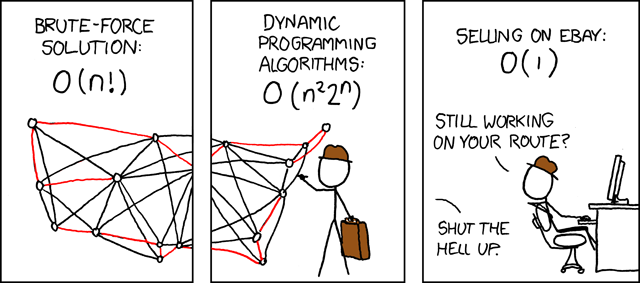
\includegraphics[height=4.5cm]{images/xkcd-tsp}
\hfill~

\rotatebox{0}{\tiny Randall Munroe, \url{http://xkcd.com/399/}, CC-BY-NC 2.5}
\end{center}}

\sectionSlide{Fragen?}

\begin{frame}\frametitle{Sprachen und Berechnung}

\begin{itemize}
\item Formale Wörter als allgemeine Abstraktion aller Daten, die in Computern verarbeitet werden können
\item Formale Sprachen als Mengen von Ein- oder Ausgaben
\item Worterkennung als allgemeine Berechnungsaufgabe
\end{itemize}

\examplebox{Beispiel: Auch die Berechnung von Funktionen kann als Wortproblem ausgedrückt werden. 
Anstatt zu fragen, "`Was ergibt $n+m$?"' kann man fragen "`Ist $n+m=r$?"'}

Daraus ergibt sich das Kernthema diese Vorlesung:\\[2ex]

\narrowcentering{\alert{Sprachen zu klassifizieren heißt Rechenaufgaben klassifizieren}}

\end{frame}

\begin{frame}\frametitle{Zwei Hierarchien}

Wir haben zwei Hierarchien von Sprachklassen kennengelernt\bigskip

\begin{enumerate}[(1)]
\item \alert{Chomsky-Hierarchie:}
\[ \text{Typ 3}\subset \text{det. kontextfrei}\subset\text{Typ 2}\subset\text{Typ 1}\subset\text{Typ 0}\]
Ansatz: natürliche Definition über Grammatiken\bigskip
\item \alert{Hierarchie der Komplexitätsklassen:}
\[\Scomplclass{L}\subseteq\Scomplclass{NL}\subseteq \Scomplclass{P}\subseteq\Scomplclass{NP}\subseteq\Scomplclass{PSpace}\subseteq \Scomplclass{Exp}\subseteq \Scomplclass{NExp}\]
Ansatz: natürliche und robuste Definition durch Beschränkung von Turingmaschinen
\end{enumerate}

\end{frame}

\begin{frame}[t]\frametitle{Eine Hierarchie?\phantom{p}}

\narrowcentering
{%
\scalebox{0.75}{%
\begin{tikzpicture}[decoration=penciline, decorate,
	mybox/.style args = {}{
		rectangle,rounded corners=5pt,minimum width=2.5cm,draw=black,fill=cyan!40,
		align=flush center
	},
	myarrow/.style args = {}{
		line width=0.4mm,
		draw=black
	}
]
\pgfmathsetseed{7729}
\path[use as bounding box] (-4,-6) rectangle (9,6); % add "draw" to see it
% \draw[help lines] (0,0) grid (5,5);

\node (nexp) [mybox=] at (0,4) {\Scomplclass{NExp}};
\node (exp) [mybox=] at (0,3) {\Scomplclass{Exp}};
\node (pspace) [mybox=] at (0,2) {\Scomplclass{PSpace}};
\node (lsavitch) [draw=none,fill=none,circle] at (1.5,2) {=};
\node (npspace) [mybox=] at (3,2) {\Scomplclass{NPSpace}};
\node (np) [mybox=] at (0,1) {\Scomplclass{NP}};
\node (p) [mybox=] at (0,0) {\Scomplclass{P}};
\node (nl) [mybox=] at (0,-1) {\Scomplclass{NL}};
\node (l) [mybox=] at (0,-2.3) {\Scomplclass{L}};

\node (re) [mybox=] at (2,5.5) {RE, Typ 0\\[-0.6ex]{\footnotesize(semi-entscheidbar, Turing-erkennbar)}};
\node (cs) [mybox=] at (4,0.5) {Typ 1, CSL\\[-0.6ex]{\footnotesize(kontextsensitiv)}};
\node (lcslspace) [draw=none,fill=none,circle] at (5.5,0.5) {=};
\node (nspacen) [mybox=] at (7,0.5) {\Scomplclass{NSpace}$(n)$};

\node (cf) [mybox=] at (4,-1) {Typ 2, CFL\\[-0.6ex]{\footnotesize(kontextfrei)}};
\node (dcf) [mybox=] at (4,-2.3) {DCFL\\[-0.6ex]{\footnotesize(det. kontextf.)}};
\node (reg) [mybox=] at (4,-3.6) {Typ 3, REG\\[-0.6ex]{\footnotesize(regulär)}};
\node (lregtime) [draw=none,fill=none,circle] at (5.5,-3.6) {=};
\node (nspacen) [mybox=] at (7,-3.6) {\Scomplclass{DSpace}$(1)$};

\draw[myarrow=] (l)--(nl);
\draw[myarrow=] (nl)--(p);
\draw[myarrow=] (p)--(np);
\draw[myarrow=] (np)--(pspace);
\draw[myarrow=] (pspace)--(exp);
\draw[myarrow=] (exp)--(nexp);
\draw[myarrow=] (nexp)--(re);

\draw[myarrow=] (reg)--(dcf);
\draw[myarrow=] (dcf)--(cf);
\draw[myarrow=] (cf)--(cs);
\draw[myarrow=] (cs)--(pspace);
\draw[myarrow=] (reg)--(l);
\draw[myarrow=] (cf)--(p);
\draw[myarrow=] (nl)--(cs);

\node (legend) [rectangle,text width=3.7cm,draw=darkred,fill=strongyellow!40,
		align=flush left] at (7.5,4) {Bekannte Beziehungen (Mengeninklusionen) zwischen den Sprachklassen; zumeist geht man von echten Teilmengen aus, aber bewiesen ist das nur in manchen Fällen};
\end{tikzpicture}}}


\end{frame}

\begin{frame}[t]\frametitle{Typische Beispiel-Sprachen}

\ghost{\hspace{2.0cm}\raisebox{6.3cm}{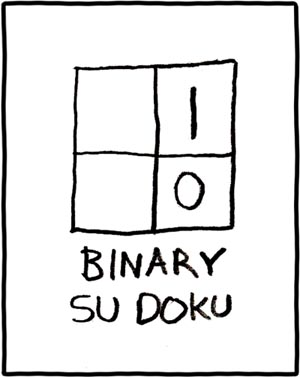
\includegraphics[height=1.5cm]{images/Sudoku-xkcd74}$*$}
\hspace{10.5cm}\raisebox{1.5cm}{\rotatebox{90}{\tiny $*$ Randall Munroe, \url{http://xkcd.com/74/}, CC-BY-NC 2.5}}}%
\narrowcentering
{%
\scalebox{0.75}{%
\begin{tikzpicture}[decoration=penciline, decorate,
	mybox/.style args = {}{
		rectangle,rounded corners=5pt,minimum width=2.5cm,draw=black,fill=cyan!40,
		align=flush center
	},
	myexbox/.style args = {}{
		rectangle,rounded corners=1pt,minimum width=2cm,draw=darkgreen,fill=darkgreen!40,
		align=flush center
	},
	myarrow/.style args = {}{
		line width=0.4mm,
		draw=black
	}
]
\pgfmathsetseed{7729}
\path[use as bounding box] (-4,-6) rectangle (9,6); % add "draw" to see it
% \draw[help lines] (0,0) grid (5,5);

\node (nexp) [mybox=] at (0,4) {\Scomplclass{NExp}};
\node (exp) [mybox=] at (0,3) {\Scomplclass{Exp}};
\node (pspace) [mybox=] at (0,2) {\Scomplclass{PSpace}};
% \node (lsavitch) [draw=none,fill=none,circle] at (1.5,2) {=};
% \node (npspace) [mybox=] at (3,2) {\Scomplclass{NPSpace}};
\node (np) [mybox=] at (0,1) {\Scomplclass{NP}};
\node (p) [mybox=] at (0,0) {\Scomplclass{P}};
\node (nl) [mybox=] at (0,-1) {\Scomplclass{NL}};
\node (l) [mybox=] at (0,-2.3) {\Scomplclass{L}};

\node (re) [mybox=] at (2,5.5) {RE, Typ 0\\[-0.6ex]{\footnotesize(semi-entscheidbar, Turing-erkennbar)}};
\node (cs) [mybox=] at (4,0.5) {Typ 1, CSL\\[-0.6ex]{\footnotesize(kontextsensitiv)}};
% \node (lsavitch) [draw=none,fill=none,circle] at (5.5,0.5) {=};
% \node (nspacen) [mybox=] at (7,0.5) {\Scomplclass{NSpace}$(n)$};

\node (cf) [mybox=] at (4,-1) {Typ 2, CFL\\[-0.6ex]{\footnotesize(kontextfrei)}};
\node (dcf) [mybox=] at (4,-2.3) {DCFL\\[-0.6ex]{\footnotesize(det. kontextf.)}};
\node (reg) [mybox=] at (4,-3.6) {Typ 3, REG\\[-0.6ex]{\footnotesize(regulär)}};
% \node (lsavitch) [draw=none,fill=none,circle] at (5.5,-3.6) {=};
% \node (nspacen) [mybox=] at (7,-3.6) {\Scomplclass{DSpace}$(1)$};

\draw[myarrow=] (l)--(nl);
\draw[myarrow=] (nl)--(p);
\draw[myarrow=] (p)--(np);
\draw[myarrow=] (np)--(pspace);
\draw[myarrow=] (pspace)--(exp);
\draw[myarrow=] (exp)--(nexp);
\draw[myarrow=] (nexp)--(re);

\draw[myarrow=] (reg)--(dcf);
\draw[myarrow=] (dcf)--(cf);
\draw[myarrow=] (cf)--(cs);
\draw[myarrow=] (cs)--(pspace);
\draw[myarrow=] (reg)--(l);
\draw[myarrow=] (cf)--(p);
\draw[myarrow=] (nl)--(cs);

\node (cslex) [myexbox=] at (6.3,0.8) {$\{\Sterm{a}^i\Sterm{b}^i\Sterm{c}^i\mid i\geq 0\}$};
\node (cslex2) [myexbox=] at (6.2,0.1) {\Slang{SAT}};
\node (cflex) [myexbox=] at (7,-0.7) {$\{\Sterm{a}^i\Sterm{b}^j\Sterm{c}^k\mid i\neq j\text{ oder }j\neq k\}$};
\node (cflex2) [myexbox=] at (6.5,-1.4) {$\{w w^r\mid w\in\{\Sterm{a},\Sterm{b}\}^*\}$};
\node (dcflex) [myexbox=] at (6,-2.3) {$\{\Sterm{a}^i\Sterm{b}^i\mid i\geq 0\}$};
\node (regex) [myexbox=] at (6.2,-3.3) {$\{\Sterm{a}^i\Sterm{b}^j\mid i,j\geq 0\}$};
\node (regex2) [myexbox=] at (7.0,-4.0) {alle endlichen Sprachen};

\node (npex) [myexbox=] at (-2.0,1.3) {\Slang{SAT}};
\node (pex) [myexbox=] at (-2.0,0.3) {\Slang{HornSAT}};
\node (pex) [myexbox=] at (5.0,4.9) {Halteproblem};

% \node (legend) [rectangle,text width=3.7cm,draw=darkred,fill=strongyellow!40,
% 		align=flush left] at (7.5,4) {Bekannte Beziehungen (Mengeninklusionen) zwischen den Sprachklassen; zumeist geht man von echten Teilmengen aus, aber bewiesen ist das nur in manchen Fällen};
\end{tikzpicture}}}

\end{frame}

\begin{frame}[t]\frametitle{Berechnungsmodelle}

\narrowcentering
{%
\scalebox{0.75}{%
\begin{tikzpicture}[decoration=penciline, decorate,
	mybox/.style args = {}{
		rectangle,rounded corners=5pt,minimum width=2.5cm,draw=black,fill=cyan!40,
		align=flush center
	},
	mymachbox/.style args = {}{
		rectangle,rounded corners=2pt,minimum width=2cm,draw=darkred,fill=darkred!40,
		align=flush center
	},
	myarrow/.style args = {}{
		line width=0.4mm,
		draw=black
	}
]
\pgfmathsetseed{7729}
\path[use as bounding box] (-4,-6) rectangle (9,6); % add "draw" to see it
% \draw[help lines] (0,0) grid (5,5);

\node (nexp) [mybox=] at (0,4) {\Scomplclass{NExp}};
\node (exp) [mybox=] at (0,3) {\Scomplclass{Exp}};
\node (pspace) [mybox=] at (0,2) {\Scomplclass{PSpace}};
% \node (lsavitch) [draw=none,fill=none,circle] at (1.5,2) {=};
% \node (npspace) [mybox=] at (3,2) {\Scomplclass{NPSpace}};
\node (np) [mybox=] at (0,1) {\Scomplclass{NP}};
\node (p) [mybox=] at (0,0) {\Scomplclass{P}};
\node (nl) [mybox=] at (0,-1) {\Scomplclass{NL}};
\node (l) [mybox=] at (0,-2.3) {\Scomplclass{L}};

\node (re) [mybox=] at (2,5.5) {RE, Typ 0\\[-0.6ex]{\footnotesize(semi-entscheidbar, Turing-erkennbar)}};
\node (cs) [mybox=] at (4,0.5) {Typ 1, CSL\\[-0.6ex]{\footnotesize(kontextsensitiv)}};
% \node (lsavitch) [draw=none,fill=none,circle] at (5.5,0.5) {=};
% \node (nspacen) [mybox=] at (7,0.5) {\Scomplclass{NSpace}$(n)$};

\node (cf) [mybox=] at (4,-1) {Typ 2, CFL\\[-0.6ex]{\footnotesize(kontextfrei)}};
\node (dcf) [mybox=] at (4,-2.3) {DCFL\\[-0.6ex]{\footnotesize(det. kontextf.)}};
\node (reg) [mybox=] at (4,-3.6) {Typ 3, REG\\[-0.6ex]{\footnotesize(regulär)}};
% \node (lsavitch) [draw=none,fill=none,circle] at (5.5,-3.6) {=};
% \node (nspacen) [mybox=] at (7,-3.6) {\Scomplclass{DSpace}$(1)$};

\draw[myarrow=] (l)--(nl);
\draw[myarrow=] (nl)--(p);
\draw[myarrow=] (p)--(np);
\draw[myarrow=] (np)--(pspace);
\draw[myarrow=] (pspace)--(exp);
\draw[myarrow=] (exp)--(nexp);
\draw[myarrow=] (nexp)--(re);

\draw[myarrow=] (reg)--(dcf);
\draw[myarrow=] (dcf)--(cf);
\draw[myarrow=] (cf)--(cs);
\draw[myarrow=] (cs)--(pspace);
\draw[myarrow=] (reg)--(l);
\draw[myarrow=] (cf)--(p);
\draw[myarrow=] (nl)--(cs);

\node (cslex) [mymachbox=] at (6.1,0.8) {LBA};
\node (cflex) [mymachbox=] at (6.2,-1.0) {PDA};
\node (dcflex) [mymachbox=] at (6.2,-2.3) {DPDA};
\node (regex) [mymachbox=] at (6.2,-3.3) {NFA};
\node (regex2) [mymachbox=] at (6.2,-4.0) {DFA};

\node (npex) [mymachbox=] at (-2.0,1.3) {Polyzeit NTM};
\node (pex) [mymachbox=] at (-2.0,0.3) {Polyzeit DTM};
\node (pex) [mymachbox=] at (5.6,4.9) {DTM};
\node (pex) [mymachbox=] at (5.6,5.5) {NTM};

% \node (legend) [rectangle,text width=3.7cm,draw=darkred,fill=strongyellow!40,
% 		align=flush left] at (7.5,4) {Bekannte Beziehungen (Mengeninklusionen) zwischen den Sprachklassen; zumeist geht man von echten Teilmengen aus, aber bewiesen ist das nur in manchen Fällen};
\end{tikzpicture}}}

\end{frame}

\begin{frame}\frametitle{Trennung der Sprachklassen}

Die Chomsky-Hierarchie ist echt. Methoden, um 
\redalert{Nicht}enthaltensein einer Sprache in einer bestimmten Hierarchieebene zu zeigen:

\begin{itemize}
\item \alert{Typ 3}: reguläres Pumping-Lemma, Myhill-Nerode-Index, Abschlusseigenschaften (V10)
\item \alert{Typ 2}: kontextfreies Pumping-Lemma (V13), Abschlusseigenschaften (V14)
\item \alert{det. Typ 2}: Abschlusseigenschaften (V16)
\item \alert{Typ 1}: Entscheidbarkeit, Abschlusseigenschaften (V19/V20)
\item \alert{Typ 0}: Semi-Entscheidbarkeit (V19/V20)
\end{itemize}

Bei den Komplexitätsklassen sind bisher weitaus weniger Unterschiede bewiesen.
Exponentielle Ressourcenzugaben erzeugen echt größere Klassen (z.B. $\Scomplclass{P}\subset\Scomplclass{Exp}$).
\medskip

\textcolor{devilscss}{Daraus folgt auch, dass $\Scomplclass{ExpSpace}$-harte Sprachen nicht kontextsensitiv sind, auch wenn sie entscheidbar sind}

\end{frame}


\newcommand{\myyes}{$\textcolor{darkgreen}{\checkmark}$}
\newcommand{\myno}{$\textcolor{darkred}{\times}$}

\begin{frame}\frametitle{Übersicht Abschlusseigenschaften}

\begin{center}
\begin{tabular}{r|ccccc|l}
	& \multicolumn{5}{c|}{Abschluss unter \ldots} &\\
Sprache & $\cap$ & $\cup$ & $\overline{\phantom{L}}$ & $\circ$ & $^*$ & Automat\\\hline
Typ 0 & \myyes & \myyes & \myno & \myyes & \myyes & TM (DTM/NTM)\\
Typ 1 & \myyes & \myyes & \myyes & \myyes & \myyes & LBA ($\stackrel{?}{=}$ det. LBA)\\
Typ 2 & \myno & \myyes & \myno & \myyes & \myyes & PDA\\
Det. Typ 2 & \myno & \myno & \myyes & \myno & \myno & DPDA\\
Typ 3 & \myyes & \myyes & \myyes & \myyes & \myyes & DFA/NFA
\end{tabular}
\end{center}

\end{frame}


\begin{frame}\frametitle{Übersicht Probleme}

Die Entscheidbarkeit verschiedener relevanter Probleme ist je nach Sprachklasse
unterschiedlich:

\begin{center}
\begin{tabular}{r|cccccc}
% 	& \multicolumn{5}{c|}{Abschluss unter \ldots} &\\
Sprache & \rotatebox{90}{Wortproblem} & \rotatebox{90}{Leerheit} & \rotatebox{90}{Äquivalenz} & \rotatebox{90}{Regularität} & \rotatebox{90}{Inklusion} & \rotatebox{90}{Schnitt}\\\hline
Typ 0 & \myno & \myno & \myno & \myno & \myno & \myno\\
Typ 1 & \myyes & \myno & \myno & \myno & \myno & \myno\\
Typ 2 & \myyes & \myyes & \myno & \myno & \myno & \myno\\
Det. Typ 2 & \myyes & \myyes & \myyes & \myyes & \myno & \myno\\
Typ 3 & \myyes & \myyes & \myyes & (\myyes) & \myyes & \myyes
\end{tabular}
\end{center}

\end{frame}

\begin{frame}\frametitle{Wortprobleme lösen}

Wie schwer ist es, dass Wortproblem zu lösen, wenn die Eingabe eine (geeignet kodierte) Sprache und ein zu testendes Wort ist?\bigskip

\narrowcentering{
\begin{tabular}{rl}
Sprache & Zeitkomplexität bzgl. Wortlänge $n$\\\hline
Typ 3 & $O(n)$ (Abarbeitung DFA)\\
Det. Typ 2 & $O(n)$ (Abarbeitung DPDA)\\
Typ 2 &  $O(n^3)$ (CYK-Algorithmus)\\
\Scomplclass{P} & polynomiell (z.B. Hyperresolution für Hornlogik)\\
\Scomplclass{NP} & exponentiell (z.B. Resolution allgemein)\\
Typ 1 & $O(n\cdot |\Gamma|^n)$ (z.B. über LBA-Konfigurationsgraph)\\
Typ 0 & unentscheidbar\\
\end{tabular}}\bigskip

Das Wortproblem für \Scomplclass{NP} und Typ 1 ist \Scomplclass{NP}-vollständig bzw. \Scomplclass{PSpace}-vollständig.
Es ist nicht bewiesen aber wahrscheinlich, dass es keine subexponentiellen Algorithmen gibt.

\end{frame}

\begin{frame}\frametitle{Nichtdeterminismus}

% \begin{itemize}
% \item
\alert{Nichtdeterministische Akzeptanzbedingung:}
\\Gibt es mindestens einen Lauf, der akzeptiert?\\
% $\leadsto$ nichtsymmetrische Bedingung!
% \item Determinisierung nicht immer klar.
% \end{itemize}
\bigskip

\narrowcentering{
\begin{tabular}{ccc}
Det. & Nichtdet. & \\[-1ex]
Automatenmodell &  Automatenmodell & äquivalent?\\\hline
DFA & NFA & \myyes \\
DPDA & PDA & \myno \\
DLBA & LBA & ? \\
DTM & NTM & \myyes \\
\end{tabular}}\bigskip

\begin{itemize}
\item Oft ist es schwierig, Nichtdeterminismus unter Ressourcenbeschränkungen aufzulösen, nicht nur bei LBAs\\
z.B. ist auch $\Scomplclass{P}\neq\Scomplclass{NP}$ offen
\item Wegen der Asymmetrie hat jede nichtdeterministische Klasse eine Komplementärklasse, die oft (vermutlich) unterschiedlich ist (z.B. \Scomplclass{coNP} vs. \Scomplclass{NP})
\end{itemize}

\end{frame}

\begin{frame}\frametitle{Ein einfacher Beweis für \Scomplclass{P} = \Scomplclass{NP} ;-)}

\begin{align*}
\text{Wir wissen:}      && \Slang{L} \in \Scomplclass{P} \quad& \text{impliziert}\quad \Slang{L} \in \Scomplclass{NP}  \\
\text{Daher gilt:}  &&          \Slang{L} \notin \Scomplclass{NP} \quad& \text{impliziert}\quad \Slang{L} \notin \Scomplclass{P}\\
\text{Anders gesagt:}  &&   \Slang{L} \in \Scomplclass{coNP} \quad& \text{impliziert}\quad \Slang{L} \in \Scomplclass{coP} \\
\text{Das heißt:} &&       \Scomplclass{coNP} &\subseteq  \Scomplclass{coP}\\
\text{Wegen $\Scomplclass{coP} = \Scomplclass{P}$ gilt:}  &&            \Scomplclass{coNP} &\subseteq \Scomplclass{P}\\
\text{Somit gilt:} &&       \Scomplclass{NP} &\subseteq \Scomplclass{P}\\
\text{D.h., wegen $\Scomplclass{P} \subseteq \Scomplclass{NP}$ gilt:} &&       \Scomplclass{NP} &= \Scomplclass{P}
\end{align*}

\mbox{}\hfill q.e.d.?

\end{frame}

% Darstellung der entsprechenden Grammatiken (wo verfügbar)
% Trennung der Sprachklassen: Methoden

% \sectionSlide{Ausblick und Anwendungen}
\frame{\begin{center}
{\LARGE
Ausblick und Anwendungen}\bigskip

~\hfill
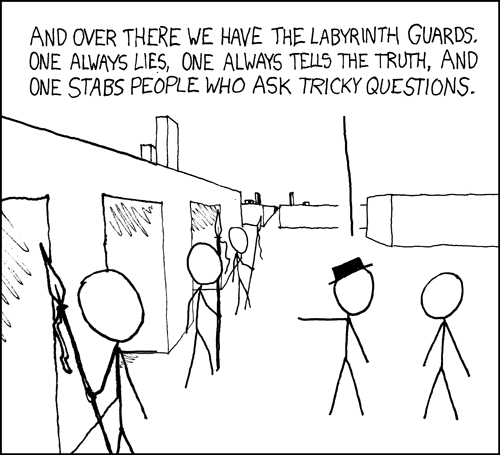
\includegraphics[height=5.5cm]{images/xkcd246-labyrinth-puzzle}
\hfill~
\rotatebox{90}{\tiny Randall Munroe, \url{http://xkcd.com/246/}, CC-BY-NC 2.5}
\end{center}}

\begin{frame}\frametitle{Formale Sprachen}

Formale Sprachen in der Praxis:
\begin{itemize}
\item Typ 3: extrem weit verbreitet in Form von regulären Ausdrücken; im \alert{Kompilerbau} als Lexer; noch einfachere Sprachen bei Anfrage/Auswahlmechanismen z.B. CSS-Selektoren
\item det. Typ 2: besonders relevant im \alert{Kompilerbau} (LR(k)-Grammatiken)
\item nichtdet. Typ 2: in der \alert{Sprachverarbeitung}; in dieser Anwendung teils auch etwas stärkere Sprachklassen (z.B. Tree-Adjoining Grammars)
\end{itemize}
Typ-1-Sprachen haben kaum praktische Anwendungen, Typ-0-Sprachen fallen mit allgemeinen TMs zusammen

\end{frame}


\begin{frame}\frametitle{Automatentheorie}

Es gibt viele Automatenmodelle jenseits der hier vorgestellten:
\begin{itemize}
\item \alert{Baumautomaten} arbeiten auf Baumstrukturen, die sie von oben oder unten her lesen
\item \alert{Automaten für unendliche Strukturen} verwenden andere Akzeptanzbedingungen, die für unendliche Abarbeitungen Sinn ergeben
\item \alert{Hybride Automaten} modellieren komplexe dynamische Systeme mithilfe von Differentialgleichungen
\item \alert{Eingeschränkte Automatenmodelle} z.B. partiell geordnete Automaten, erkennen spezielle reguläre Sprachen
\item \ldots
\end{itemize}
Wesentliche Anwendungen von Automaten:
\begin{itemize}
\item Definition "`interessanter"' Sprachklassen
\item Lösung algorithmischer Probleme (z.B. Inklusionstest von Sprachen)
\end{itemize}

\end{frame}

\begin{frame}\frametitle{Logik}

Aussagenlogik ist nur der Anfang \ldots

\begin{itemize}
\item \alert{Prädikatenlogik/Logik erster Stufe} erweitert die Struktur atomarer Aussagen (Prädikate, Terme, Variablen, \ldots); Quantoren $\forall$ und $\exists$ ermöglichen es, sich auf viele Aussagen zu beziehen ohne alle einzeln zu nennen
\item \alert{Logik zweiter Stufe} führt zudem Variablen für Prädikate und entsprechende Quantoren ein
\end{itemize}
$\leadsto$ Ausgangspunkt vieler anwendungsspezifischer Logiken
\bigskip

Wesentliche Anwendungen:
\begin{itemize}
\item Wissensrepräsentation
\item Logikprogrammierung
\item Constraint-Erfüllungsprobleme
\item Verifikation
\end{itemize}

\end{frame}

\begin{frame}\frametitle{Logisches Schließen}

Großes Fachgebiet; sehr stark anwendungsspezifisch
\bigskip

Nennenswerte Klassen stark optimierter Logiktools:

\begin{itemize}
\item SAT-Solver: aussagenlogisches Schließen
\item Theorembeweiser: Entwickeln formaler Beweise in sehr ausdrucksstarken Logiken
\item Model-Checker: effiziente Verifikation von formalen Aussagen bzgl. abstrakter Programmmodelle
\item Logikprogramm-Systeme: Berechnung der Ergebnisse logischer Programme verschiedenster Form
\item Ontologie-Reasoner: Anfragebeantwortung über logischen Wissensbasen und Datenbanken
\end{itemize}

\end{frame}

\begin{frame}\frametitle{}

~\hspace{-1.6cm}
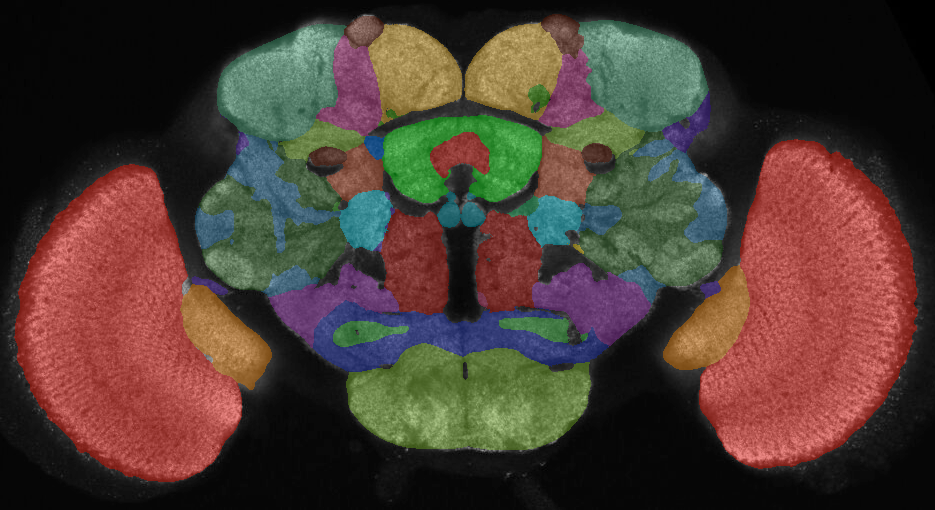
\includegraphics[width=16.1cm]{images/fly-brain}

\end{frame}

\begin{frame}\frametitle{Komplexitätstheorie}

Großes Gebiet in der theoretischen Informatik, mit zwei wesentlichen Bedeutungen:

\begin{enumerate}[1]
\item \alert{Eigenständiges Forschungsgebiet}, das sich vielen grundlegenden Fragen widmet (einschl. $\Scomplclass{P}\neq\Scomplclass{NP}?$); Theorie der Kryptographie; Quantenkomplexität
% 
\item \alert{Methoden für andere Forschungsfelder}, welche die komplexitätstheoretische Analyse von Problemen
in vielen Fachgebieten ermöglichen; Themen wie parametrisierte Komplexität oder Ausgabekomplexität sind aus
Anwendungen motiviert
\end{enumerate}

Weiteres Fachgebiet: \redalert{Berechenbarkeitstheorie} (Klassifikation unentscheidbarer Probleme, alternative Berechnungsmodelle)

\end{frame}

% 
% Weiterführende Themen
% % Formale Sprachen (?)
% % Automatentheorie (Baumauomaten, Hybride Automaten, quantitative Modelle, ...)
% % Komplexitätstheorie (Beziehungen zwischen Komplexitätsklassen, ...)
% % Berechenbarkeitstheorie (unentscheidbare Probleme, weitere Unterteilung des Unentscheidbaren)
% % Kompilerbau
% % logikbasierte KR
% % Verifikation
% % Alternative Berechnungsmodelle: z.B. Quantumcomputing
%
% Weiterführende Vorlesungen
% % Theoretische Informatik und Logik
% % Deduction Systems
% % Advanced Logic
% % Datenbanken -- Grundlagen
% % Intelligente Systeme
% % Complexity Theory
% % Database Theory
% % Foundations of Semantic Web Technologies
% % was zu Verifikation?

\begin{frame}\frametitle{TheoLog}

Im nächsten Semester gibt es \alert{"`Theoretische Informatik und Logik"'} {\tiny(Pflicht für einige, offen für alle)}\medskip

Hören Sie die großen Fragen der Mathematik -- und die Antworten der Informatik!
\begin{itemize}
\item \redalert{Berechenbarkeit}
\begin{itemize}
\item Fleißige Biber und manch Unentscheidbares
\item Von Turingmaschinen zu Programmen
\end{itemize}
\item \redalert{Komplexität}
\begin{itemize}
\item NP: Spiele für eine Person
\item PSpace: einfache Spiele für zwei
\end{itemize}
\item \redalert{Prädikatenlogik}
\begin{itemize}
\item Die Sprache der Mathematik
\item Resolution reloaded
\item Endliche Modelle (besser bekannt als ``Datenbanken'')
\end{itemize}
\item \redalert{Mathematikerinnen als Programmiererinnen}
\begin{itemize}
\item Die Grenzen der Mathematik
\item Gödel, Turing und der ganze Rest
\end{itemize}
\end{itemize}

\end{frame}

\sectionSlide{Fragen?}

\begin{frame}\frametitle{Zusammenfassung}

\redalert{Formale Sprachen} sind die Grundlage zahlreicher Forschungs- und Anwendungsfelder der Informatik.
\bigskip

\redalert{Berechnungsmodelle} erlauben uns, allgemeine Aussagen über die Schwere und Lösbarkeit
von Berechnungsaufgaben zu treffen
\bigskip

\redalert{Formale Logik} wird als Spezifikationssprache für (zumeist anspruchsvolle) Probleme in vielen Gebieten verwendet
\bigskip

\anybox{strongyellow}{
Offene Fragen:
\begin{itemize}
\item Haben Sie noch inhaltliche Fragen?
\item Haben Sie sich ausreichend auf die Prüfung vorbereitet?
\item Sonstiges Feedback?
\end{itemize}
}


\end{frame}

\end{document}
